\documentclass{article}
\usepackage[utf8]{inputenc}
\usepackage{minted, graphicx, hyperref}

\begin{document}

\begin{center}
{\LARGE\bf COMP3013 Coursework: Design Report}\\
\vspace{2mm}
{\bf Matthew Lapointe, Takeaki Yamasaki, Zhengyi Yang}\\
\vspace{1mm}
\textbf{18th March 2016}
\end{center}

\section{YouTube Video}

\url{https://www.youtube.com/}

\section{Entity Relationship Diagram}

\begin{figure}[!h]
\begin{center}
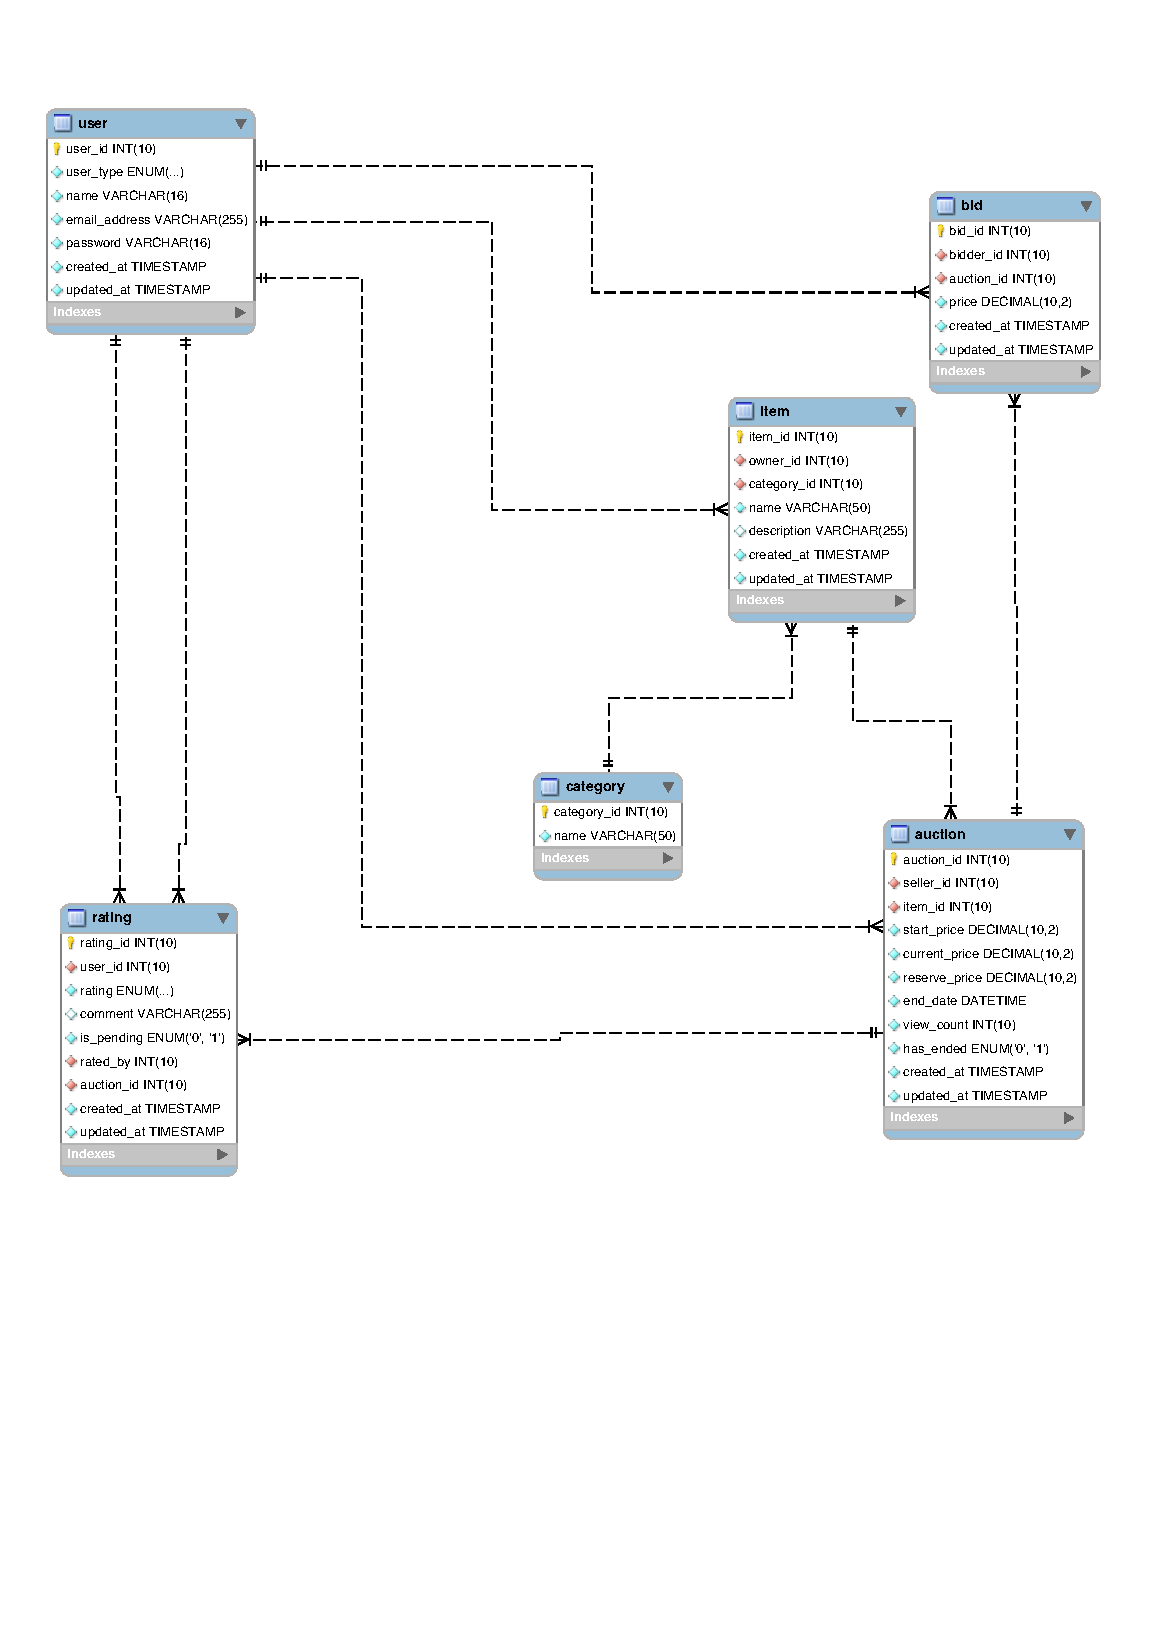
\includegraphics[scale=.65]{ERDiagram.pdf}
\end{center}
\end{figure}

\section{Database Schema}

This schema implements the ER diagram shown above. \texttt{user} and \texttt{category} are strong entities, while \texttt{item}, \texttt{auction}, \texttt{bid}, and \texttt{rating} are weak entities, with appropriate foreign key attributes. \texttt{user} to \texttt{item}, \texttt{user} to \texttt{auction}, \texttt{user} to \texttt{bid}, \texttt{user} to \texttt{rating}, and \texttt{auction} to \texttt{bid} are all one to many relationships.\\
\\
user (\underline{user\_id}, user\_type, name, email\_address, password, created\_at, updated\_at)\\
\\
item (\underline{item\_id}, owner\_id \textbf{references} user(user\_id), category\_id \textbf{references} category(category\_id), name, description, created\_at, updated\_at)\\
\\
auction (\underline{auction\_id}, seller\_id \textbf{references} user(user\_id), item\_id \textbf{references} item(item\_id), start\_price, current\_price, reserve\_price, end\_date, view\_count, has\_ended, created\_at, updated\_at)\\
\\
bid (\underline{bid\_id}, bidder\_id \textbf{references} user(user\_id), auction\_id \textbf{references} auction(auction\_id), price, created\_at, updated\_at)\\
\\
category (\underline{category\_id}, name)\\
\\
rating (\underline{rating\_id}, user\_id \textbf{references} user(user\_id), rating, comment, is\_pending, rated\_by \textbf{references} user(user\_id), auction\_id \textbf{references} auction(auction\_id), created\_at, updated\_at)

\section{Normalisation Analysis}

The schema has been implemented in SQL, thus is necessary does not contain repeating groups. The database is in First Normal Form.\\
\\
There are no tables containing composite keys, so it must be the case that each non-primary key attribute is fully functionally dependent on its primary key. The database, then, is in Second Normal Form.\\
\\
Examining the non-primary key attributes of each table, it is clear that no transitive dependencies exist. The database is in Third Normal Form.

\section{Database Queries}

\subsection{Registering and Logging In}
\begin{minted}[]{sql}
select * from user where email_address='".$email_address."'
and password='".$password."' and user_type='".$user_type."';
\end{minted}
This query retrieves entries in the \texttt{user} table which match the email address, password, and user type (seller/buyer) selected. This allows for authentication of a user attempting to log in.

\begin{minted}[]{sql}
insert into user(name,email_address,password,user_type,created_at)
values('".$name."','".$email_address."','".$password."','".$user_type."',NULL);
\end{minted}
This query inserts a new user into the database.

\subsection{Creating Auctions}
\begin{minted}[]{sql}
insert into item(owner_id, category_id, name, description, created_at)
values('".$_SESSION['user_id']."','".$item_category."','".$item_name."',
'".$item_desc."',NULL);
\end{minted}
This query inserts a new item into the \texttt{item} table.

\begin{minted}[]{sql}
insert into auction(seller_id, item_id, start_price, current_price,
reserve_price, end_date, has_ended, created_at)
values('".$_SESSION['user_id']."','".$item['item_id']."','".$start_price."',
'".$start_price."','".$reserve_price."','".$end_date."','0',NULL);
\end{minted}
This query inserts creates a new entry in the \texttt{auction} table.

\subsection{Browsing Auctions}
\begin{minted}[]{sql}
select i.item_id, i.name, i.description
from item as i
left join auction as a
on i.item_id=a.item_id
where i.category_id='".$_GET['category']."' and a.has_ended='0'
order by ".$sort.";
\end{minted}
This query retrieves all items on auction in the selected category. It arranges items by the selected criterion.

\subsection{Handling Bids}
\begin{minted}[]{sql}
select * from bid where auction_id='".$auction['auction_id']."';
order by price desc
\end{minted}
This query retrieves all the bids placed in a given auction.

\begin{minted}[]{sql}
insert into bid(bidder_id, auction_id, price, created_at)
values('".$_SESSION['user_id']."','".$auction['auction_id']."',
'".$bid_price."',NULL)
\end{minted}
This query inserts a new bid into the \texttt{bid} table.

\begin{minted}[]{sql}
select a.auction_id, i.name as item_name, i.item_id, u.user_id as seller_id,
u.name as seller_name, u.email_address as seller_address, a.reserve_price
from auction as a
left join item as i
on i.item_id = a.item_id
left join user as u
on u.user_id = a.seller_id
where end_date <= now() and has_ended='0';
\end{minted}
This query is run periodically, retrieving auctions which have ended. The item is then awarded to the user who placed the highest bid, if that bid exceeds the reserve price.

\subsection{Watching Auctions}
\begin{minted}[]{sql}
select b.price, u.user_id, u.name, u.email_address
from bid as b
left join user as u
on b.bidder_id=u.user_id
where b.auction_id=".$auction['auction_id']."
order by b.price desc
limit 1;
\end{minted}
When a new bid is placed, this query retrieves the previously highest bid, if it exists. An email is then sent to that user notifying them that they have been outbid.

\subsection{Seller Reports}
\begin{minted}[]{sql}
select a.end_date, a.current_price, a.reserve_price,
a.auction_id, a.view_count, i.name
from auction as a
left join item as i
on a.item_id = i.item_id
where a.seller_id = '".$seller['user_id']."' and a.end_date > now();
\end{minted}
This query retrieves auctions for a given seller which have not yet ended. The information is then sent to the user in an update email.

\subsection{Ratings}
\begin{minted}[]{sql}
select * from rating where user_id='".$_GET['user']."' and is_pending='0';
\end{minted}
This query retrieves from the \texttt{rating} table all ratings for a given user, which are displayed on their user page.

\begin{minted}[]{sql}
select round(avg(case rating
                 when '5' then 5
                 when '4' then 4
                 when '3' then 3
                 when '2' then 2
                 when '1' then 1
                 else null end),1) avg_rating
 from rating
 where user_id='".$_GET['user']."' and is_pending='0';
\end{minted}
This query computes the average rating for a given user, which is displayed on their user page.

\subsection{Recommendations}
\begin{minted}[]{sql}
SELECT * 
FROM auction
WHERE auction.auction_id
IN (

SELECT bid.auction_id
FROM bid
WHERE bid.bidder_id
IN (

SELECT bid.bidder_id
FROM bid
WHERE bid.bidder_id <> $user_id 
AND bid.auction_id
IN (

SELECT bid.auction_id
FROM bid
WHERE bid.bidder_id = $user_id
GROUP BY bid.auction_id
)
GROUP BY bid.bidder_id
)
GROUP BY bid.auction_id
)
AND auction.has_ended =  '0'
LIMIT 10
\end{minted}
This query provides recommendations for user by retrieving the sorts of auctions other people, who have also bid on the sorts of auctions the user have previously bid on, are currently bidding on.

\end{document}
